%-------------------------------------------------------------------------------
\section{Introduction}
\label{s:intro}
%-------------------------------------------------------------------------------

Many microservices contend with varying load as well as being \textit{latency
critical} (LC), meaning they have strict Service Level Objectives (SLOs) that
guarantee uptime and caps on the response latency of the service. However, when
developers want to run microservices, cloud systems like AWS ec2 or Kubernetes
require them to give a fixed amount of resources the service will need, \ie{} a
number of CPUs and an amount of memory~\cite{aws-ec2-resources,
kubernetes-resources}. As a result, developers choose those requirements based
on the expected peak load, and the resources are rarely fully used~\cite{borg,
nu, overprovision}.

Other tasks do not fall into this category: \textit{best effort} (BE) tasks such
as long-running map reduce jobs or background data analytics do not have an SLO.

Indeed, many cloud scheduling systems separate the work they run into classes,
that include one class for LC tasks, which have resource requirements, and one
class for BE tasks, which don't. This includes distributed schedulers, \eg{}
Borg\cite{borg} or Kubernetes\cite{kubernetes-resources}, and single machine
schedulers, for example Caladan\cite{caladan}.

Splitting workloads into LC and BE is popular because it allows providers to run
BE tasks on machines reserved for LC tasks that are currently experiencing low
load and thus have idle resources~\cite{perfiso}. However, enforcing strict
isolation is challenging: Should an LC service experience a spike in load, it
needs to be able to immediately have access to all the resources it had
reserved. Any delay likely leads to violations of the services SLOs.

\begin{figure}[t]
    \centering
    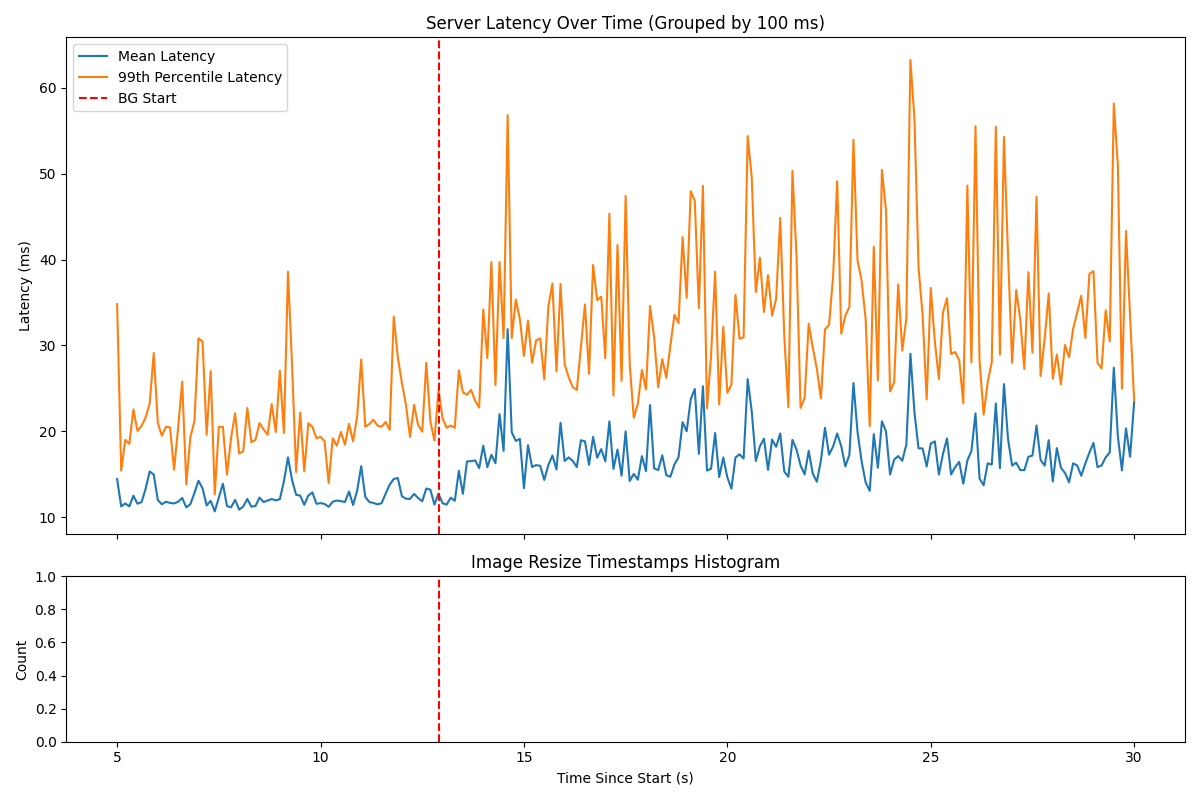
\includegraphics[width=\columnwidth]{graphs/kubernetes-unedited.png}
    \caption{E2E repsonse times for a simple social network web application,
    before and after starting load on a BE
    service}\label{fig:kubernetes-unedited}
\end{figure}

Current popular systems fail to properly isolate latency critical from best
effort workloads. When running a small but realistic social network web
application on Kubernetes, we observe significant impacts on its latency when
starting a best effort workload, doing image resizing, on the same machine.
\autoref{fig:kubernetes-unedited} plots the end-to-end latency of an endpoint
that gets a users feed on the top graph; the bottom graph shows the throughput
of the BE workload. The mean response latency jumps from $\sim$7ms to
$\sim$15ms, and the 99th percentile latency from $\sim$10ms to $\sim$23ms. 

Understanding where the isolation fails requires understanding the underlying
mechanism that is enforcing it: Linux's \cgroups{}. \cgroups{} offers an API to
enforce isolation of multiple resources inclduing memory and CPU, but this work
will focus on CPU isolation. Most modern containers rely on \cgroups{} for CPU
isolation; this includes all Open Container Initiative (OCI) compliant
containers, including Kubernetes but also Docker, CRI-O, and
containerd~\cite{oci-cgroups,docker-docs-cgroups,container-isolation-article}.
VM frameworks, including Firecracker, AFaas and libvirt, also rely on \cgroups{}
to manage CPU time allocation when the number of vCPUs is
oversubscribed.~\cite{firecracker-cgroups,afaas,libvirt-cgroups}

The part of the \cgroups{} interface that these systems use to isolate LC and BE
is based on weight: each workload is put into its own group, and each group is
assigned a weight in the range [1, 10000]. \cgroups{} specifies that each group
gets CPU time proportional to its weight as a share of the sum of weights of
runnable groups~\cite{cgroups-kerneldocs}.\footnote{Other operating systems use
a similar interface, for instance Windows exposes a number of shares.} For
instance, if two groups $cg1$ and $cg2$ have weights 200 and 300 respectively,
when they are both active their CPU time ratio should also be $2:3$. However, if
$cg1$ has no runnable threads, then $cg2$ would represent 100\% of the runnable
weight and get all the CPU time.

However, as \autoref{fig:kubernetes-unedited} showed, something is going wrong:
the effect the BE has on the latency of the LC server is much higher than
expected for something with $1/10000$th of its weight. As we show in more detail
in \autoref{s:problem}, the problem that leads to the increased latencies
observed is that Linux will run a BE process on one core, unaware that an LC
process is runnable and waiting on another. This happens because Linux uses
per-CPU runqueues. Doing so avoids the synchronization overhead of having a
global runqueue, but also means that enforcing weights across the runqueues
properly requires expensive synchronization. A key challenge this work addresses
is how to manage this tension between expensive synchronization and affecting
strict isolation across cores.\hmng{I don't really talk about 2.3 here}

Our approach addresses this challenge by exposing in the API and enforcing in
the scheduler a categorical split between LC and BE. As we show in
\autoref{ss:approach:solves-problems}, a categorical split makes it viable to
enforce the isolation across cores, because it reduces the number of times the
scheduler is required to synchronize across cores. Enforcing weights across
cores requires the scheduler to synchronize every scheduling tick, but with a
categorical separation it only has to do so on \textit{event} - every time a
core starts running a BE process, and every time it queues an LC task.

A challenge that emerges from such categorical separation is that, when the LC
is under high load, the BE processes need somewhere to go. Killing them should
only be a last resort, but as we show in \autoref{ss:eval:parking}, running them
even for small amounts of time can impact LC server performance.

We address this challenge by making the split between LC and BE as strict as
possible without crashing the BE processes. When the CPU utilization is high
enough that any amount of running a BE would interfere with an LC, we enable BEs
to exist in an ephemeral state called \textit{parked}, which does the minimal
amount of work required to keep the BEs from crashing. In order to do this, the
scheduler ensures that the userspace process doens't run and consume resources,
but the kernelspace handlers that manage TCP connections and timers on behalf of
the BE processes still run. Discussed further in \autoref{ss:approach:parking},
the parked state represents a compromise of doing the least amount of work
required to stop BEs from crashing or dying.

We implement such a strict and catorgical separation in Liinux, and show that it
is able to significiantly improve Linux's ability to isolate LC from BE
workloads: in the same Kubernetes experiment, the increase in average latency
when starting a BE workload goes from $>$2x to 0. The contributions of this
paper are thus as follows: 
\begin{enumerate}
    \item identifying the reason isolation of LC from BE often fails is that
    \cgroups{} does a poor job of enforcing the weights of different groups
    across cores; and that this dramatically affects end-to-end latencies
    \item showing that BEs can get no userpace CPU time for extended periods of
    time and stay alive and keep running after; and that doing so enables LC
    workloads to perform much better under high load than if they are throttled,
    \item implement in Linux \schedbe{}, a new class for BE tasks that is
    categorically separate from the default class LC tasks run in, which
    isolates LC workloads from BE ones and minimizes the amount of cross-core
    checks required, and naturally enforces the parked state
\end{enumerate}
